\section{Study 2: independent targets and strong competitors}
\label{sec:study2}

Study~2 evaluated \STwoTargetsTotal\ targets (between \STwoTargetsMin\ and
\STwoTargetsMax\ per benchmark, one per strict cluster) under the frozen plan of
Section~\ref{sec:design2}. Table~\ref{tab:study2} lists every decision,
Table~\ref{tab:study2banks} the main contrasts per benchmark, and
Table~\ref{tab:study2policies} the policy means. \StudyTwoSummary

\IfFileExists{tables/study2.tex}{\begin{table}[tbp]
\centering\footnotesize
\caption{Study 2: decisions under the frozen plan (primary panel size $N=8$; one target per strict family cluster). Holm sig.: benchmarks with a Holm-significant difference favouring EOST-M / favouring the competitor (Holm over the 88 superiority tests); positive: benchmarks on which EOST-M is better; median: median over benchmarks of the relative improvement of EOST-M (\%; for C3 the relative difference of the posterior-draw marginal (PDM) Bayesian CAT, for C5a the range of coverage). Supported: at least five benchmarks for EOST-M and none against (C3: equivalence on at least six; C5a: inside on at least six). $^\ast$C5a, C5b and C6 concern EOST-M's recalibrated interval.}
\label{tab:study2}
\setlength{\tabcolsep}{3pt}
\begin{tabular}{@{}lllcccl@{}}
\toprule
 & EOST-M versus & Endpoint & Holm sig. & positive & median & Supported \\
\midrule
R2 & plug-in 2PL (MFI:pi) & log loss & 5/0 & 8/8 & $+5.9$ & yes \\
R3 & Naive & score IAE & 6/0 & 8/8 & $+53.9$ & yes \\
R4 & plug-in 2PL (MFI:pi) & $|\mathrm{cov}-0.9|$ & 5/0 & 8/8 & $+41.6$ & yes \\
C1 & Rasch-type plug-in & log loss & 5/0 & 7/8 & $+2.4$ & yes \\
C2 & Rasch-type marginal & log loss & 4/0 & 8/8 & $+1.8$ & no \\
C4 & Random:mg & score IAE & 4/0 & 8/8 & $+21.1$ & no \\
C5b & raw EOST-M interval$^\ast$ & interval score & 0/2 & 4/8 & $+1.0$ & no \\
C6 & Naive (Wilson)$^\ast$ & interval score & 6/0 & 7/8 & $+35.0$ & yes \\
C7 & ATLAS-style 3PL CAT & score IAE & 4/0 & 8/8 & $+26.0$ & no \\
C8 & tinyBenchmarks & error @50 & 4/0 & 8/8 & $+29.6$ & no \\
C9 & MINCE & error @50 & 5/0 & 8/8 & $+44.8$ & yes \\
\midrule
C3 & PDM Bayesian CAT (equivalence) & log loss & \multicolumn{2}{c}{4/8 within $\pm$1\%} & $+0.32$ & no \\
C5a & (coverage in $[0.85,0.95]$)$^\ast$ & coverage & \multicolumn{2}{c}{5/8 banks inside} & 0.81--0.91 & no \\
\bottomrule
\end{tabular}
\end{table}
}{}
\IfFileExists{tables/study2_policies.tex}{\begin{table}[tbp]
\centering\footnotesize
\caption{Study 2: policy means at $N=8$ averaged over the eight benchmarks: integrated held-out log loss, integrated absolute score error, mean coverage and width of the 90\% score interval, and integrated interval score ($\alpha=0.1$; lower is better). Recalibrated intervals share the estimates of the raw policy.}
\label{tab:study2policies}
\setlength{\tabcolsep}{4pt}
\begin{tabular}{@{}lccccc@{}}
\toprule
Policy & log loss & score IAE & coverage & width & interval score \\
\midrule
EOST-M (EIG:mg) & 0.3582 & 0.0324 & 0.74 & 0.095 & 0.201 \\
EOST-M, recalibrated & (same) & 0.0324 & 0.86 & 0.134 & 0.206 \\
Rasch-type plug-in (MFI:1pr) & 0.3680 & 0.0344 & 0.81 & 0.121 & 0.220 \\
Rasch-type, recalibrated & (same) & 0.0344 & 0.91 & 0.271 & 0.321 \\
Rasch-type marginal (EIG:1prmg) & 0.3660 & 0.0366 & 0.82 & 0.128 & 0.214 \\
PDM Bayesian CAT, BMI (frozen burn-in) & 0.3599 & 0.0339 & 0.76 & 0.101 & 0.221 \\
PDM Bayesian CAT, EIG (frozen burn-in) & 0.3589 & 0.0326 & 0.77 & 0.101 & 0.210 \\
plug-in 2PL (MFI:pi) & 0.3825 & 0.0352 & 0.59 & 0.076 & 0.304 \\
ATLAS-style 3PL CAT & 0.3825 & 0.0448 & 0.48 & 0.085 & 0.417 \\
Random:mg & 0.3651 & 0.0422 & 0.88 & 0.162 & 0.211 \\
Naive (Wilson) & -- & 0.0640 & 0.90 & 0.235 & 0.290 \\
EOST-M, cross-fitted EB & 0.3583 & 0.0319 & 0.74 & 0.094 & 0.197 \\
EOST-M, Student-$t$ EB & 0.3601 & 0.0319 & 0.70 & 0.088 & 0.212 \\
mixed (every 4th random) & 0.3583 & 0.0326 & 0.77 & 0.102 & 0.189 \\
\bottomrule
\end{tabular}
\end{table}
}{}

\subsection{Replication with independent targets}
With one target per cluster, EOST-M's held-out log loss was lower than plug-in Fisher
CAT's on \STwoRTwoPos\ of 8 benchmarks (median \STwoRTwoMed\%), Holm-significantly on
\STwoRTwoFav\ and in favour of the baseline on \STwoRTwoBase: replication R2 is
\STwoRTwoVerdict. Its score error was \STwoRThreeMed\% below that of naive subsampling
(R3, \STwoRThreeVerdict; \STwoRThreeFav\ benchmarks significant), and its intervals were
less miscalibrated than plug-in Fisher CAT's by a median of \STwoRFourMed\% (R4,
\STwoRFourVerdict). \StudyTwoReplicationText

\IfFileExists{tables/study2_banks.tex}{\begin{table}[tbp]
\centering\footnotesize
\caption{Study 2 per benchmark ($N=8$): number of targets (independent clusters) and relative improvement (\%) of EOST-M over each competitor; * Holm-significant. $^\dagger$Recorded aggregate verdicts.}
\label{tab:study2banks}
\setlength{\tabcolsep}{4pt}
\begin{tabular}{@{}lrrrrrr@{}}
\toprule
 & & \multicolumn{3}{c}{held-out log loss} & \multicolumn{2}{c}{score IAE} \\
\cmidrule(lr){3-5}\cmidrule(l){6-7}
Benchmark & targets & MFI:pi & Rasch plug-in & Rasch marg. & Random:mg & ATLAS \\
\midrule
GSM8K & 40 & $+5.3$* & $+1.7$ & $+0.3$ & $+22.0$* & $+3.4$ \\
ARC-C & 40 & $+4.5$ & $+2.0$* & $+1.7$* & $+12.8$ & $+51.2$* \\
HellaSwag & 40 & $+12.2$* & $+6.4$* & $+1.3$ & $+43.1$* & $+38.0$* \\
WinoGrande & 40 & $+5.3$* & $+2.8$* & $+3.2$* & $+30.0$* & $+48.7$* \\
MMLU & 40 & $+7.2$* & $+4.7$* & $+5.0$* & $+5.0$ & $+24.1$ \\
SWE-bench V. & 40 & $+6.9$* & $+1.8$ & $+2.1$* & $+20.2$ & $+16.3$* \\
LiveCodeBench$^\dagger$ & 15 & $+6.4$ & $+3.4$* & $+1.9$ & $+46.7$* & $+27.9$ \\
CRUXEval-O$^\dagger$ & 12 & $+5.4$ & $-0.4$ & $+0.2$ & $+2.0$ & $+1.4$ \\
\bottomrule
\end{tabular}
\end{table}
}{}

\subsection{Integration, constraint, and Bayesian CATs}\label{sec:s2fb}
Against the regularized Rasch-type plug-in test, EOST-M's held-out log loss was lower on
\STwoCOnePos\ of 8 benchmarks (median \STwoCOneMed\%; \STwoCOneFav\ Holm-significant for
EOST-M, \STwoCOneBase\ for the competitor): C1 is \STwoCOneVerdict. Against the same
one-parameter model integrated over its item posterior, the median improvement was
\STwoCTwoMed\% (\STwoCTwoFav/\STwoCTwoBase; C2 \STwoCTwoVerdict). \StudyTwoRaschText
\par
The posterior-draw marginal (PDM) Bayesian CAT, which also integrates the calibrators'
abilities and the hyperprior through posterior draws, differed from EOST-M by a median of \STwoCThreeMed\% in held-out log loss and
was practically equivalent within $\pm1\%$ on \STwoCThreeEq\ of 8 benchmarks (C3
\STwoCThreeVerdict; Table~\ref{tab:equiv}). \StudyTwoFBText

\StudyTwoFBDetails

\IfFileExists{tables/fbfix.tex}{\begin{table}[tbp]
\centering\footnotesize
\caption{Study 2, Bayesian CATs against EOST-M at $N=8$ (post hoc correction of the burn-in and exploratory joint model; same targets, panels, holdouts and chains). Equivalence: 90\% bootstrap interval of the relative difference in held-out log loss within $\pm1\%$ (rule of C3: at least six benchmarks); median relative difference of log loss (positive: Bayesian CAT worse); benchmarks with a Holm-significant difference favouring EOST-M / the Bayesian CAT; the same for the score error (median relative improvement of EOST-M); mean coverage of the 90\% score interval (EOST-M: 0.74).}
\label{tab:fbfix}
\setlength{\tabcolsep}{3pt}
\begin{tabular}{@{}lcccccc@{}}
\toprule
 & \multicolumn{3}{c}{held-out log loss} & \multicolumn{2}{c}{score IAE} & \\
\cmidrule(lr){2-4}\cmidrule(lr){5-6}
Variant & equiv. & median \% & sig. & median \% & sig. & coverage \\
\midrule
PDM Bayesian, BMI (frozen, burn-in 10) & 4/8 & $+0.32$ & 0/0 & $+5.1$ & 0/0 & 0.76 \\
PDM Bayesian, EIG (frozen, burn-in 10) & 5/8 & $+0.18$ & 0/0 & $-0.8$ & 0/0 & 0.77 \\
PDM Bayesian, BMI (burn-in 60) & 3/8 & $+0.39$ & 0/0 & $+5.0$ & 0/0 & 0.76 \\
PDM Bayesian, EIG (burn-in 60) & 3/8 & $+0.50$ & 0/0 & $+4.2$ & 0/0 & 0.76 \\
joint fully Bayesian, BMI (exploratory) & 5/8 & $+0.33$ & 0/0 & $+2.8$ & 0/0 & 0.74 \\
joint fully Bayesian, EIG (exploratory) & 5/8 & $+0.05$ & 0/0 & $-1.5$ & 0/0 & 0.75 \\
\bottomrule
\end{tabular}
\end{table}
}{}
\IfFileExists{tables/equivalence.tex}{\begin{table}[tbp]
\centering\footnotesize
\caption{Study 2, hypothesis C3: relative difference (\%) of held-out log loss of the posterior-draw marginal (PDM) Bayesian CAT (Bayesian maximum information) with respect to EOST-M at $N=8$, its 90\% bootstrap interval over targets, and equivalence within $\pm1\%$.}
\label{tab:equiv}
\begin{tabular}{@{}lrcc@{}}
\toprule
Benchmark & difference & 90\% interval & equivalent \\
\midrule
GSM8K & +1.31 & [-0.71, +3.27] & no \\
ARC-C & +0.29 & [-0.12, +0.73] & yes \\
HellaSwag & +0.09 & [-0.32, +0.49] & yes \\
WinoGrande & -0.06 & [-0.28, +0.16] & yes \\
MMLU & +0.26 & [-0.20, +0.69] & yes \\
SWE-bench V. & +0.56 & [-0.02, +1.10] & no \\
LiveCodeBench & +0.99 & [-0.30, +2.27] & no \\
CRUXEval-O & +0.35 & [-0.81, +1.61] & no \\
\bottomrule
\end{tabular}
\end{table}
}{}
\IfFileExists{tables/fbfix_N4.tex}{\begin{table}[tbp]
\centering\footnotesize
\caption{Study 2, Bayesian CATs against EOST-M at $N=4$ (post hoc correction of the burn-in and exploratory joint model; same targets, panels, holdouts and chains). Equivalence: 90\% bootstrap interval of the relative difference in held-out log loss within $\pm1\%$ (rule of C3: at least six benchmarks); median relative difference of log loss (positive: Bayesian CAT worse); benchmarks with a Holm-significant difference favouring EOST-M / the Bayesian CAT; the same for the score error (median relative improvement of EOST-M); mean coverage of the 90\% score interval (EOST-M: 0.78).}
\label{tab:fbfixfour}
\setlength{\tabcolsep}{3pt}
\begin{tabular}{@{}lcccccc@{}}
\toprule
 & \multicolumn{3}{c}{held-out log loss} & \multicolumn{2}{c}{score IAE} & \\
\cmidrule(lr){2-4}\cmidrule(lr){5-6}
Variant & equiv. & median \% & sig. & median \% & sig. & coverage \\
\midrule
PDM Bayesian, BMI (frozen, burn-in 10) & 4/8 & $+0.33$ & 0/0 & $+2.6$ & 0/0 & 0.82 \\
PDM Bayesian, EIG (frozen, burn-in 10) & 4/8 & $+0.45$ & 0/0 & $+6.5$ & 0/0 & 0.79 \\
PDM Bayesian, BMI (burn-in 60) & 4/8 & $+0.21$ & 0/0 & $+1.6$ & 0/0 & 0.81 \\
PDM Bayesian, EIG (burn-in 60) & 2/8 & $+0.45$ & 1/0 & $+5.8$ & 1/0 & 0.79 \\
joint fully Bayesian, BMI (exploratory) & 4/8 & $-0.03$ & 0/0 & $+1.0$ & 0/0 & 0.79 \\
joint fully Bayesian, EIG (exploratory) & 4/8 & $+0.17$ & 0/0 & $-0.8$ & 0/0 & 0.79 \\
\bottomrule
\end{tabular}
\end{table}
}{}

\subsection{Adaptivity and benchmark-reduction methods}\label{sec:s2red}
All methods below use the same eight calibrators per target. ATLAS and tinyBenchmarks were
designed for panels of hundreds to thousands of systems, so these comparisons concern the
small-panel regime, not the methods in their native settings; MINCE targets few calibration
models. Under the same calibrated model, adaptive selection reduced the score error of random
items by a median of \STwoCFourMed\% (C4 \STwoCFourVerdict; \STwoCFourFav\ benchmarks
significant). Against the ATLAS-style 3PL CAT the median improvement in score error was
\STwoCSevenMed\% (C7 \STwoCSevenVerdict). After 50 items, EOST-M's score error was
\STwoCEightMed\% below tinyBenchmarks' gp-IRT (C8 \STwoCEightVerdict) and \STwoCNineMed\%
below MINCE's subset mean (C9 \STwoCNineVerdict); Table~\ref{tab:reduction} gives the
errors at 25, 50 and 100 items. \StudyTwoReductionText

\IfFileExists{tables/reduction.tex}{\begin{table}[tbp]
\centering\footnotesize
\caption{Study 2: absolute error of the full-bank score (percentage points) after 25, 50 and 100 items at $N=8$, averaged over targets and benchmarks. tinyBenchmarks and MINCE select their items without adapting to the target.}
\label{tab:reduction}
\begin{tabular}{@{}lccc@{}}
\toprule
Method & 25 items & 50 items & 100 items \\
\midrule
EOST-M (EIG:mg) & 3.39 & 2.81 & 2.13 \\
ATLAS-style 3PL CAT & 4.46 & 4.20 & 3.79 \\
Random:mg & 4.78 & 3.34 & 2.42 \\
tinyBenchmarks gp-IRT & 4.96 & 4.39 & 4.49 \\
tinyBenchmarks p-IRT & 4.69 & 3.92 & 3.31 \\
tinyBenchmarks anchors & 6.23 & 5.62 & 5.37 \\
MINCE subset mean & 6.71 & 4.69 & 3.19 \\
Naive (Wilson) & 7.05 & 4.88 & 3.26 \\
\bottomrule
\end{tabular}
\end{table}
}{}
\IfFileExists{tables/tiny_audit.tex}{\begin{table}[tbp]
\centering\footnotesize
\caption{Study 2, post hoc audit of tinyBenchmarks at $N=8$: percentage of cells (target $\times$ replicate) in which fewer anchor items than the budget were available: K-Means returns at most one anchor per distinct item embedding, and with eight calibrators the embeddings take only as many distinct values as there are distinct response patterns among the items, often fewer than 100; last column: median number of anchors actually used at a budget of 100.}
\label{tab:tinyaudit}
\begin{tabular}{@{}lcccc@{}}
\toprule
 & \multicolumn{3}{c}{cells with fewer anchors than budget (\%)} & anchors used \\
\cmidrule(lr){2-4}
Benchmark & 25 & 50 & 100 & at budget 100 \\
\midrule
GSM8K & 1 & 7 & 76 & 82 \\
ARC-C & 0 & 0 & 0 & 100 \\
HellaSwag & 0 & 0 & 29 & 100 \\
WinoGrande & 0 & 0 & 1 & 100 \\
MMLU & 0 & 0 & 0 & 100 \\
SWE-bench V. & 0 & 2 & 100 & 71 \\
LiveCodeBench & 0 & 0 & 98 & 67 \\
CRUXEval-O & 0 & 0 & 8 & 100 \\
\bottomrule
\end{tabular}
\end{table}
}{}

\subsection{Calibrated uncertainty}\label{sec:s2cov}
\StudyTwoCoverageText

\IfFileExists{figures/study2_coverage.pdf}{%
\begin{figure}[tbp]
\centering
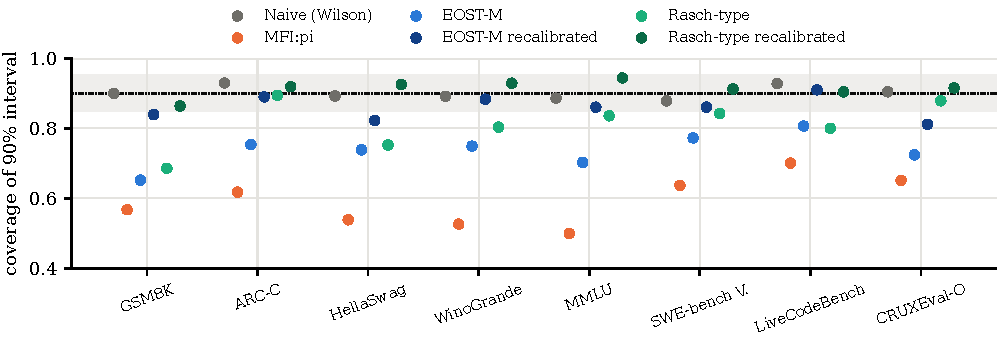
\includegraphics[width=\linewidth]{figures/study2_coverage.pdf}
\caption{Study 2: coverage of the 90\% score interval per benchmark at $N=8$ (mean over steps, replicates and targets). Shaded band: the $[0.85,0.95]$ criterion of hypothesis C5a; dotted: nominal.}
\label{fig:study2cov}
\end{figure}}{}

\subsection{Temporal validation and robustness}\label{sec:s2rob}
\StudyTwoRobustText

\subsection{Robustness of the empirical-Bayes hyperprior}\label{sec:eb}
The empirical-Bayes hyperprior is load-bearing: with a fixed weakly-informative prior,
the study-1 gain of EOST-M over plug-in Fisher CAT halves (Section~\ref{sec:sensitivity}).
Because it is estimated from the same panel, it could act as an opportunistic tuning
parameter. Stability and predictive checks (post hoc) and three alternatives run in study~2
under its frozen plan address this.

\paragraph{Stability.} Hyperparameters are re-estimated on bootstrap resamples of the items
(abilities held fixed), on two random halves of the items, and at $N=8$ on bootstrap
resamples of the calibrators (Table~\ref{tab:ebstab}). Resampling items moves them by at most
\EBItemsSdMaxEight\ (standard deviation, $N=8$): they pool hundreds of items and are well
determined given the panel. What varies is the panel: resampling calibrators moves the
spread of the log-discriminations by \EBCalSdSigmaA\ and that of the difficulties by
\EBCalSdSigmaB, comparable to the variation between panels (\EBBetweenSigmaA\ for
$\sigma_a$). The hyperprior therefore reflects which systems are in the panel, not noise
in the items.

\IfFileExists{tables/eb_stability.tex}{\begin{table}[tbp]
\centering\footnotesize
\caption{Stability of the empirical-Bayes hyperparameters (post hoc; three panels per benchmark and panel size). Medians over benchmarks of: the standard deviation across panels (between), the bootstrap standard deviation over items with abilities fixed (items), the absolute difference between fits on two random halves of the items (halves), and at $N=8$ the bootstrap standard deviation over calibrators (calibrators).}
\label{tab:ebstab}
\setlength{\tabcolsep}{3pt}
\begin{tabular}{@{}lccccccccc c@{}}
\toprule
 & \multicolumn{3}{c}{$N=4$} & \multicolumn{3}{c}{$N=8$} & \multicolumn{3}{c}{$N=16$} & $N=8$ \\
\cmidrule(lr){2-4}\cmidrule(lr){5-7}\cmidrule(lr){8-10}\cmidrule(l){11-11}
 & between & items & halves & between & items & halves & between & items & halves & calibrators \\
\midrule
$\mu_b$ & 0.17 & 0.09 & 0.16 & 0.07 & 0.07 & 0.11 & 0.08 & 0.07 & 0.07 & 0.10 \\
$\sigma_b$ & 0.11 & 0.09 & 0.10 & 0.16 & 0.07 & 0.10 & 0.18 & 0.07 & 0.05 & 0.15 \\
$\mu_a$ & 0.06 & 0.05 & 0.06 & 0.08 & 0.04 & 0.07 & 0.07 & 0.04 & 0.04 & 0.14 \\
$\sigma_a$ & 0.05 & 0.03 & 0.05 & 0.05 & 0.03 & 0.03 & 0.04 & 0.03 & 0.04 & 0.06 \\
\bottomrule
\end{tabular}
\end{table}
}{}

\paragraph{Prior predictive checks.} For each of the \PPCPanels\ panels (three per benchmark
and panel size), 200 response matrices were simulated from the fitted hyperprior given the
calibrators' abilities and compared with the observed matrix on three statistics; under a
correct model about 5\% of the two-sided predictive $p$-values would fall below 0.05. The
share of items that every calibrator or no calibrator answers correctly matters most for
Proposition~\ref{prop:cap}, because such items are located by the prior alone. It is
reproduced on average (median observed \PPCExtremeObs, simulated \PPCExtremeSim) but not
panel by panel: $p<0.05$ for \PPCExtremeLow\% of the panels (observed share higher than
simulated in \PPCExtremeAbove\%, lower in \PPCExtremeBelow\%), most of them on
HellaSwag and MMLU. The spread of the items' proportions correct is reproduced (observed
\PPCSdPObs, simulated \PPCSdPSim; $p<0.05$ for \PPCSdPLow\%). The mean item--rest
correlation is mostly lower than simulated (observed \PPCRestObs, simulated \PPCRestSim;
$p<0.05$ for \PPCRestLow\% of the panels, \PPCRestBelow\% below and \PPCRestAbove\% above),
again mainly on the multiple-choice banks of the Open LLM Leaderboard: real systems agree
with each other less, item by item, than a unidimensional 2PL with independent items
implies. The hyperprior therefore captures the distribution of item locations on which
EOST-M relies, while the response model is misspecified in its dependence structure, one
reason why model-based score intervals are too narrow (Section~\ref{sec:s2cov}).

\paragraph{Leave-item-block-out, other families, hierarchical Bayes.} Study~2 ran EOST-M
with a cross-fitted hyperprior (estimated, for every item, on the other half of the items,
so that no item informs its own prior) and with Student-$t$ hyperprior families ($\nu=4$) for
both item parameters; the Bayesian CATs integrate the hyperparameters instead of plugging
them in, which is the hierarchical Bayesian benchmark. Relative to EOST-M, the cross-fitted
variant left held-out log loss unchanged (median relative difference \SecXfVsEostMedAbs\%) and
the Student-$t$ variant made it slightly worse on every benchmark (median
\SecTpVsEostMedAbs\%), with no benchmark significant, and the Bayesian CATs were not
significantly different on any benchmark (Section~\ref{sec:s2fb}). The gain of
EOST-M therefore does not come from fitting the prior to the very items it is applied to,
nor from the Gaussian family or the plug-in hyperparameters.
